\documentclass[11pt]{article}

\usepackage[margin=1in]{geometry}
\usepackage[T1]{fontenc}
\usepackage[utf8]{inputenc}
\usepackage{lmodern}
\usepackage{microtype}
\usepackage{booktabs}
\usepackage{longtable}
\usepackage{graphicx}
\usepackage{float}
\usepackage{caption}
\usepackage{subcaption}
\usepackage{array}
\usepackage{xcolor}
\usepackage{hyperref}
\usepackage{enumitem}
\usepackage{siunitx}
\usepackage{fancyhdr}

\hypersetup{
  colorlinks=true,
  linkcolor=blue,
  urlcolor=blue,
  pdftitle={Task 1 Report: Lookup and Insertion Performance of BTree, DynamicPGM, and LIPP},
  pdfauthor={Cursor Cloud Agent}
}

\pagestyle{fancy}
\fancyhf{}
\lhead{COS568 Learned Index Project}
\rhead{Task 1 Report}
\cfoot{\thepage}

\title{Task 1 Report:\\Lookup and Insertion Performance of BTree, DynamicPGM, and LIPP}
\author{Prepared from committed benchmark artifacts in the repository}
\date{\today}

\begin{document}
\maketitle

\begin{abstract}
This report documents Task 1 of the COS568 Learned Index project using the benchmark
artifacts committed in this repository. The task asks us to compare the lookup and
insertion behavior of three indexes---BTree, DynamicPGM, and LIPP---on the Facebook,
Books, and OSMC 100M uint64 datasets under four prescribed workloads. We summarize what
the assignment required, what was executed for this milestone, how configurations were
selected from the raw CSV outputs, and what the recorded results show about throughput
and index size. Across the three datasets, LIPP is overwhelmingly best for read-heavy
workloads, DynamicPGM is best for insertion-heavy workloads, and BTree is the most
stable but never the top performer on either extreme. That performance split is paired
with a large size tradeoff: DynamicPGM is the most compact, BTree is modestly larger,
and LIPP uses much more memory in every dataset and workload.
\end{abstract}

\section{Assignment context and Task 1 objective}

The project studies \emph{learned indexes}: data structures that model the mapping from
keys to positions in sorted data rather than relying only on classical tree navigation.
The repository README frames two milestones. Task 1 is the measurement and comparison
baseline; Task 2 then builds a hybrid design on top of the insights from Task 1.

For Task 1, the assignment requires the following:
\begin{itemize}[leftmargin=1.5em]
    \item understand the codebase and the benchmark pipeline in \texttt{scripts/},
    \item evaluate lookup and insertion performance of BTree, DynamicPGM, and LIPP,
    \item use the Facebook, Books, and OSMC 100M uint64 datasets,
    \item run the provided workloads with three repetitions each,
    \item compare average throughput across methods and explain the observed differences,
    \item choose the best hyperparameter setting for BTree and DynamicPGM for each
    dataset/workload pair.
\end{itemize}

The four workloads described in the assignment are:
\begin{enumerate}[leftmargin=1.5em]
    \item \textbf{Lookup-only}: 2M lookups with a 50\% negative lookup ratio.
    \item \textbf{Insert-Lookup (50/50)}: 1M inserts followed by 1M lookups, with
    50\% negative lookups in the lookup phase. The benchmark reports both insert
    throughput and post-insert lookup throughput.
    \item \textbf{Mixed workload with 10\% inserts}: insertions and lookups are mixed,
    and the benchmark reports a single mixed throughput value.
    \item \textbf{Mixed workload with 90\% inserts}: again mixed, but insertion-heavy.
\end{enumerate}

The assignment also notes that BTree and DynamicPGM are run with multiple
hyperparameter settings. For each dataset/workload pair, the best-performing row is the
one with the highest average throughput across the three repeats.

\section{What we did for Task 1}

The committed summary file (\texttt{TASK1\_SUMMARY.txt}) records the Task 1 workflow that
was carried out:
\begin{itemize}[leftmargin=1.5em]
    \item downloaded the Facebook, Books, and OSMC 100M uint64 datasets,
    \item generated the four Task 1 workloads for each dataset,
    \item built the benchmark binary,
    \item ran the full sweep of 3 datasets $\times$ 3 indexes $\times$ 4 workloads with
    3 repeats each,
    \item selected, for each index and workload, the row with the highest average
    throughput across those three runs.
\end{itemize}

The benchmark outputs are stored in \texttt{results/*.csv}, and previous aggregated
throughput summaries were committed under \texttt{analysis\_results/*.csv}. For this
report, I regenerated report assets directly from the raw result CSVs so that the tables
and figures in the PDF are derived from the committed benchmark data rather than copied
manually.

\section{Methodology used in this report}

\subsection{Inputs}
The report uses only repository artifacts already committed for Task 1:
\begin{itemize}[leftmargin=1.5em]
    \item the project description in \texttt{README.md},
    \item the recorded benchmark summary in \texttt{TASK1\_SUMMARY.txt},
    \item the raw benchmark CSVs in \texttt{results/},
    \item the benchmark driver logic in \texttt{scripts/run\_benchmarks.sh}.
\end{itemize}

\subsection{Selection rule}
For each dataset and workload:
\begin{enumerate}[leftmargin=1.5em]
    \item read every result row for an index,
    \item compute the arithmetic mean throughput over the three reported repeats,
    \item select the row with the highest average throughput for that index,
    \item record the chosen row's throughput, standard deviation, index size, and
    hyperparameter setting.
\end{enumerate}

This matches the rule stated in both the assignment and the committed summary.

\subsection{Reported metrics}
The report compares:
\begin{itemize}[leftmargin=1.5em]
    \item \textbf{Throughput} in Mops/s for each required workload,
    \item \textbf{Index size} in GiB using the \texttt{index\_size\_bytes} field from the
    selected best-throughput configuration.
\end{itemize}

Throughput is the primary Task 1 metric, but index size is included because the
assignment context emphasizes that learned indexes can trade space for speed, and the
Task 1 request specifically asked for a comparison of throughput \emph{and} index size.

\section{Throughput comparison}

Table~\ref{tab:throughput} gives the best average throughput for each dataset/workload
pair, with the top method in each row shown in bold.

\begin{table}[H]
    \centering
    \caption{Best average throughput (Mops/s) from the committed Task 1 results.}
    \label{tab:throughput}
    \small
    \begin{tabular}{llrrr}
\toprule
Dataset & Workload & BTree & DynamicPGM & LIPP \\
\midrule
Facebook & Lookup-only & 1.694 & 1.797 & \textbf{358.300} \\
Facebook & Insert throughput (50/50) & 1.059 & \textbf{6.192} & 1.378 \\
Facebook & Lookup after insert (50/50) & 1.546 & 0.471 & \textbf{349.263} \\
Facebook & Mixed throughput (10\% insert) & 1.470 & 0.849 & \textbf{13.488} \\
Facebook & Mixed throughput (90\% insert) & 1.082 & \textbf{2.799} & 2.158 \\
\midrule
Books & Lookup-only & 1.690 & 1.947 & \textbf{361.350} \\
Books & Insert throughput (50/50) & 1.084 & \textbf{6.124} & 2.291 \\
Books & Lookup after insert (50/50) & 1.572 & 0.530 & \textbf{358.773} \\
Books & Mixed throughput (10\% insert) & 1.477 & 0.935 & \textbf{17.526} \\
Books & Mixed throughput (90\% insert) & 1.058 & \textbf{2.972} & 2.855 \\
\midrule
OSMC & Lookup-only & 2.063 & 1.804 & \textbf{307.095} \\
OSMC & Insert throughput (50/50) & 1.032 & \textbf{5.332} & 0.933 \\
OSMC & Lookup after insert (50/50) & 1.826 & 0.455 & \textbf{253.168} \\
OSMC & Mixed throughput (10\% insert) & 1.641 & 0.948 & \textbf{10.447} \\
OSMC & Mixed throughput (90\% insert) & 1.046 & \textbf{2.663} & 1.621 \\
\bottomrule
\end{tabular}

\end{table}

The most important pattern is immediate:
\begin{itemize}[leftmargin=1.5em]
    \item \textbf{LIPP dominates all read-heavy workloads.} It is the best method for
    lookup-only, post-insert lookup, and mixed throughput with only 10\% inserts on
    every dataset.
    \item \textbf{DynamicPGM dominates insertion-heavy workloads.} It is the best method
    for insert throughput in the 50/50 workload and for the mixed workload with 90\%
    inserts on every dataset.
    \item \textbf{BTree is consistent but never best.} It stays in a narrow performance
    band across workloads, but it does not win any row in Table~\ref{tab:throughput}.
\end{itemize}

The overall averages across the three datasets, shown in
Table~\ref{tab:overall-throughput}, reinforce the same conclusion.

\begin{table}[H]
    \centering
    \caption{Overall average throughput across the three datasets.}
    \label{tab:overall-throughput}
    \small
    \begin{tabular}{lrrr}
\toprule
Workload & BTree & DynamicPGM & LIPP \\
\midrule
Lookup-only & 1.816 & 1.849 & \textbf{342.249} \\
Insert throughput (50/50) & 1.058 & \textbf{5.882} & 1.534 \\
Lookup after insert (50/50) & 1.648 & 0.486 & \textbf{320.401} \\
Mixed throughput (10\% insert) & 1.529 & 0.911 & \textbf{13.821} \\
Mixed throughput (90\% insert) & 1.062 & \textbf{2.812} & 2.211 \\
\bottomrule
\end{tabular}

\end{table}

Several headline comparisons summarize the scale of these differences:
\begin{itemize}[leftmargin=1.5em]
    \item In the lookup-only workload, LIPP averages \SI{342.249}{Mops/s}, versus
    \SI{1.849}{Mops/s} for DynamicPGM and \SI{1.816}{Mops/s} for BTree.
    \item Relative to BTree, LIPP is about \textbf{188.5$\times$ faster} on average for
    lookup-only and about \textbf{9.0$\times$ faster} for the mixed workload with only
    10\% inserts.
    \item For 50/50 insert throughput, DynamicPGM averages \SI{5.882}{Mops/s}, which is
    about \textbf{5.6$\times$ faster} than BTree and about \textbf{3.8$\times$ faster}
    than LIPP.
    \item For the 90\% insert mixed workload, DynamicPGM still leads at
    \SI{2.812}{Mops/s}, ahead of LIPP at \SI{2.211}{Mops/s} and BTree at
    \SI{1.062}{Mops/s}.
\end{itemize}

Figure~\ref{fig:throughput} visualizes the same throughput results. The log-scale y-axis
is necessary because LIPP's lookup throughput is hundreds of Mops/s while the other
indexes stay near single-digit Mops/s.

\begin{figure}[H]
    \centering
    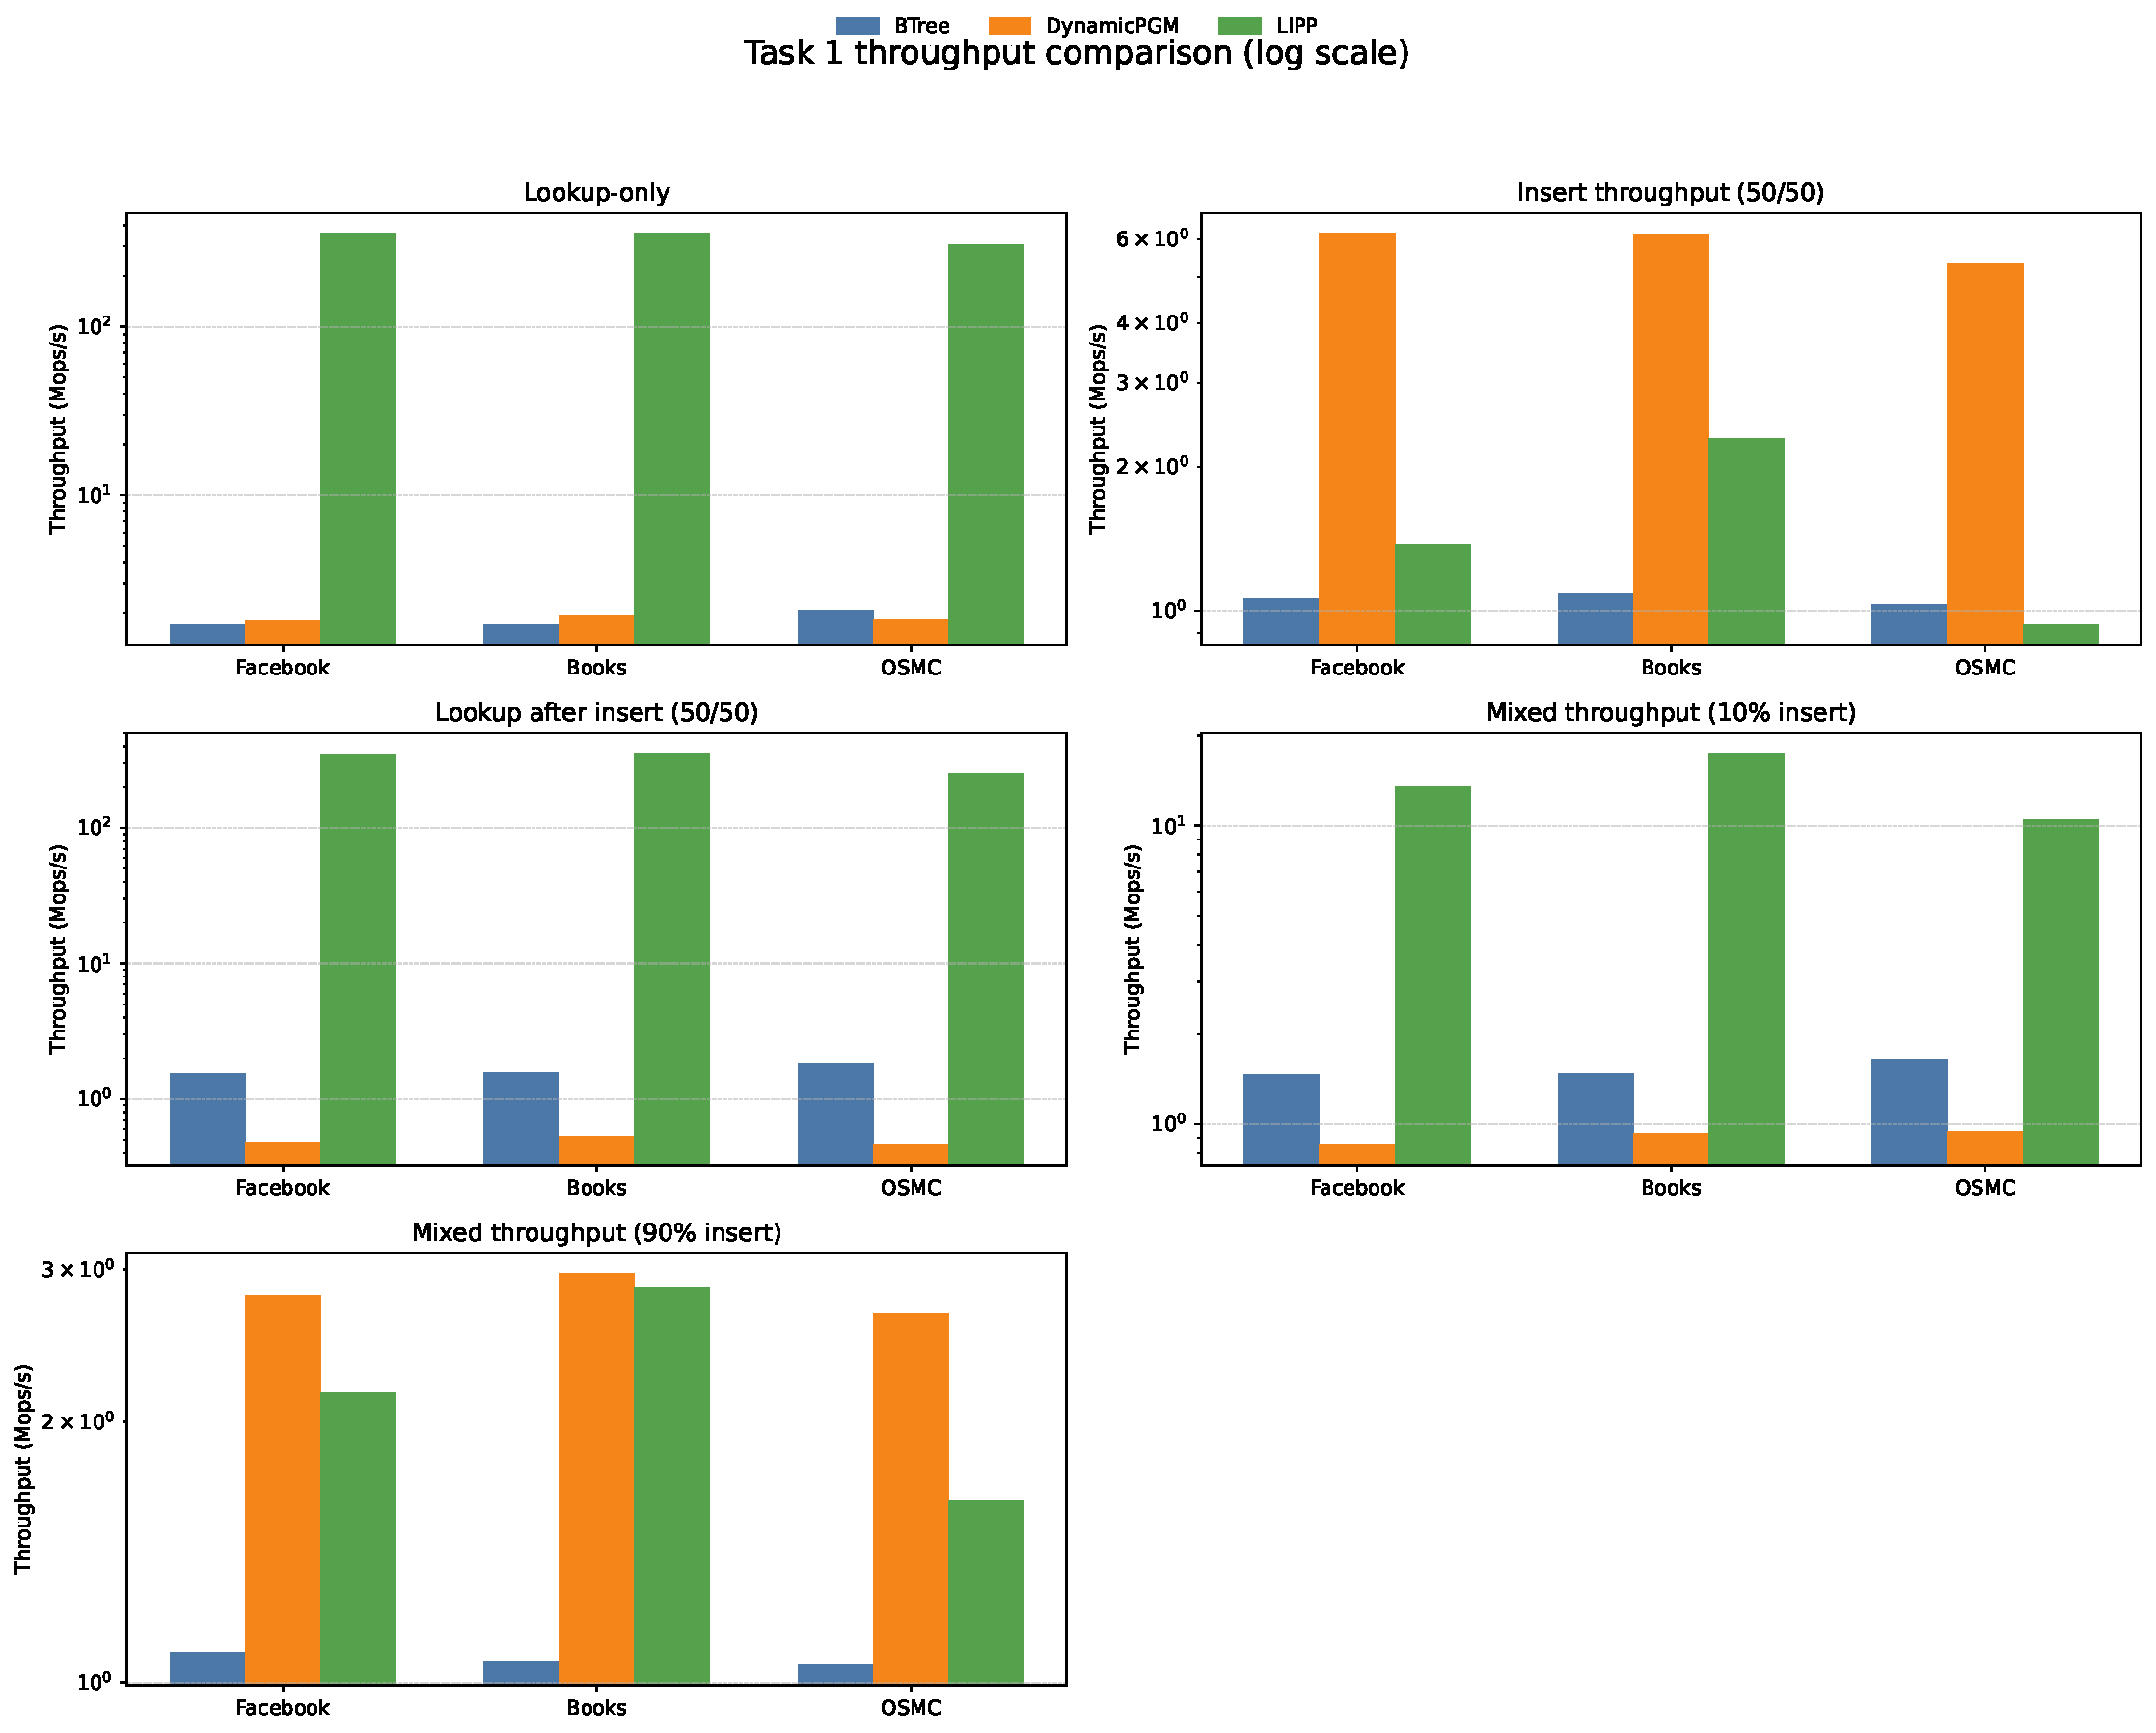
\includegraphics[width=\textwidth]{figures/task1_throughput_overview.png}
    \caption{Throughput comparison for all Task 1 workloads and datasets (log scale).}
    \label{fig:throughput}
\end{figure}

\section{Index size comparison}

Table~\ref{tab:size} compares the size of the selected best-throughput configuration in
each dataset/workload pair. Here, the smallest index size in each row is shown in bold.

\begin{table}[H]
    \centering
    \caption{Index size (GiB) of the selected best-throughput configuration.}
    \label{tab:size}
    \small
    \begin{tabular}{llrrr}
\toprule
Dataset & Workload & BTree & DynamicPGM & LIPP \\
\midrule
Facebook & Lookup-only & 1.73 & \textbf{1.60} & 11.83 \\
Facebook & Insert throughput (50/50) & 2.05 & \textbf{1.58} & 11.81 \\
Facebook & Lookup after insert (50/50) & 2.05 & \textbf{1.58} & 11.81 \\
Facebook & Mixed throughput (10\% insert) & 1.82 & \textbf{1.59} & 11.83 \\
Facebook & Mixed throughput (90\% insert) & 2.34 & \textbf{1.59} & 11.79 \\
\midrule
Books & Lookup-only & 1.73 & \textbf{1.60} & 11.01 \\
Books & Insert throughput (50/50) & 2.05 & \textbf{1.58} & 10.98 \\
Books & Lookup after insert (50/50) & 2.05 & \textbf{1.58} & 10.98 \\
Books & Mixed throughput (10\% insert) & 1.82 & \textbf{1.59} & 11.01 \\
Books & Mixed throughput (90\% insert) & 2.20 & \textbf{1.59} & 10.95 \\
\midrule
OSMC & Lookup-only & 1.73 & \textbf{1.60} & 19.21 \\
OSMC & Insert throughput (50/50) & 2.05 & \textbf{1.58} & 19.10 \\
OSMC & Lookup after insert (50/50) & 2.05 & \textbf{1.58} & 19.10 \\
OSMC & Mixed throughput (10\% insert) & 1.82 & \textbf{1.59} & 19.19 \\
OSMC & Mixed throughput (90\% insert) & 2.20 & \textbf{1.58} & 19.01 \\
\bottomrule
\end{tabular}

\end{table}

The size pattern is much more stable than the throughput pattern:
\begin{itemize}[leftmargin=1.5em]
    \item \textbf{DynamicPGM is always the most compact.} Across all selected
    configurations it stays near \SI{1.58}{GiB} to \SI{1.60}{GiB}.
    \item \textbf{BTree is moderately larger.} It ranges from about \SI{1.73}{GiB} to
    \SI{2.34}{GiB}, averaging \SI{1.98}{GiB}.
    \item \textbf{LIPP is dramatically larger.} It ranges from about \SI{10.95}{GiB} to
    \SI{19.21}{GiB}, averaging \SI{13.97}{GiB}.
\end{itemize}

This means LIPP's speed advantage comes with a substantial memory cost. Averaged across
all selected configurations, LIPP is about \textbf{8.8$\times$ larger} than DynamicPGM
and about \textbf{7.1$\times$ larger} than BTree. The gap is even larger on OSMC: in the
lookup-only workload, LIPP is about \textbf{12.0$\times$ larger} than DynamicPGM.

\begin{figure}[H]
    \centering
    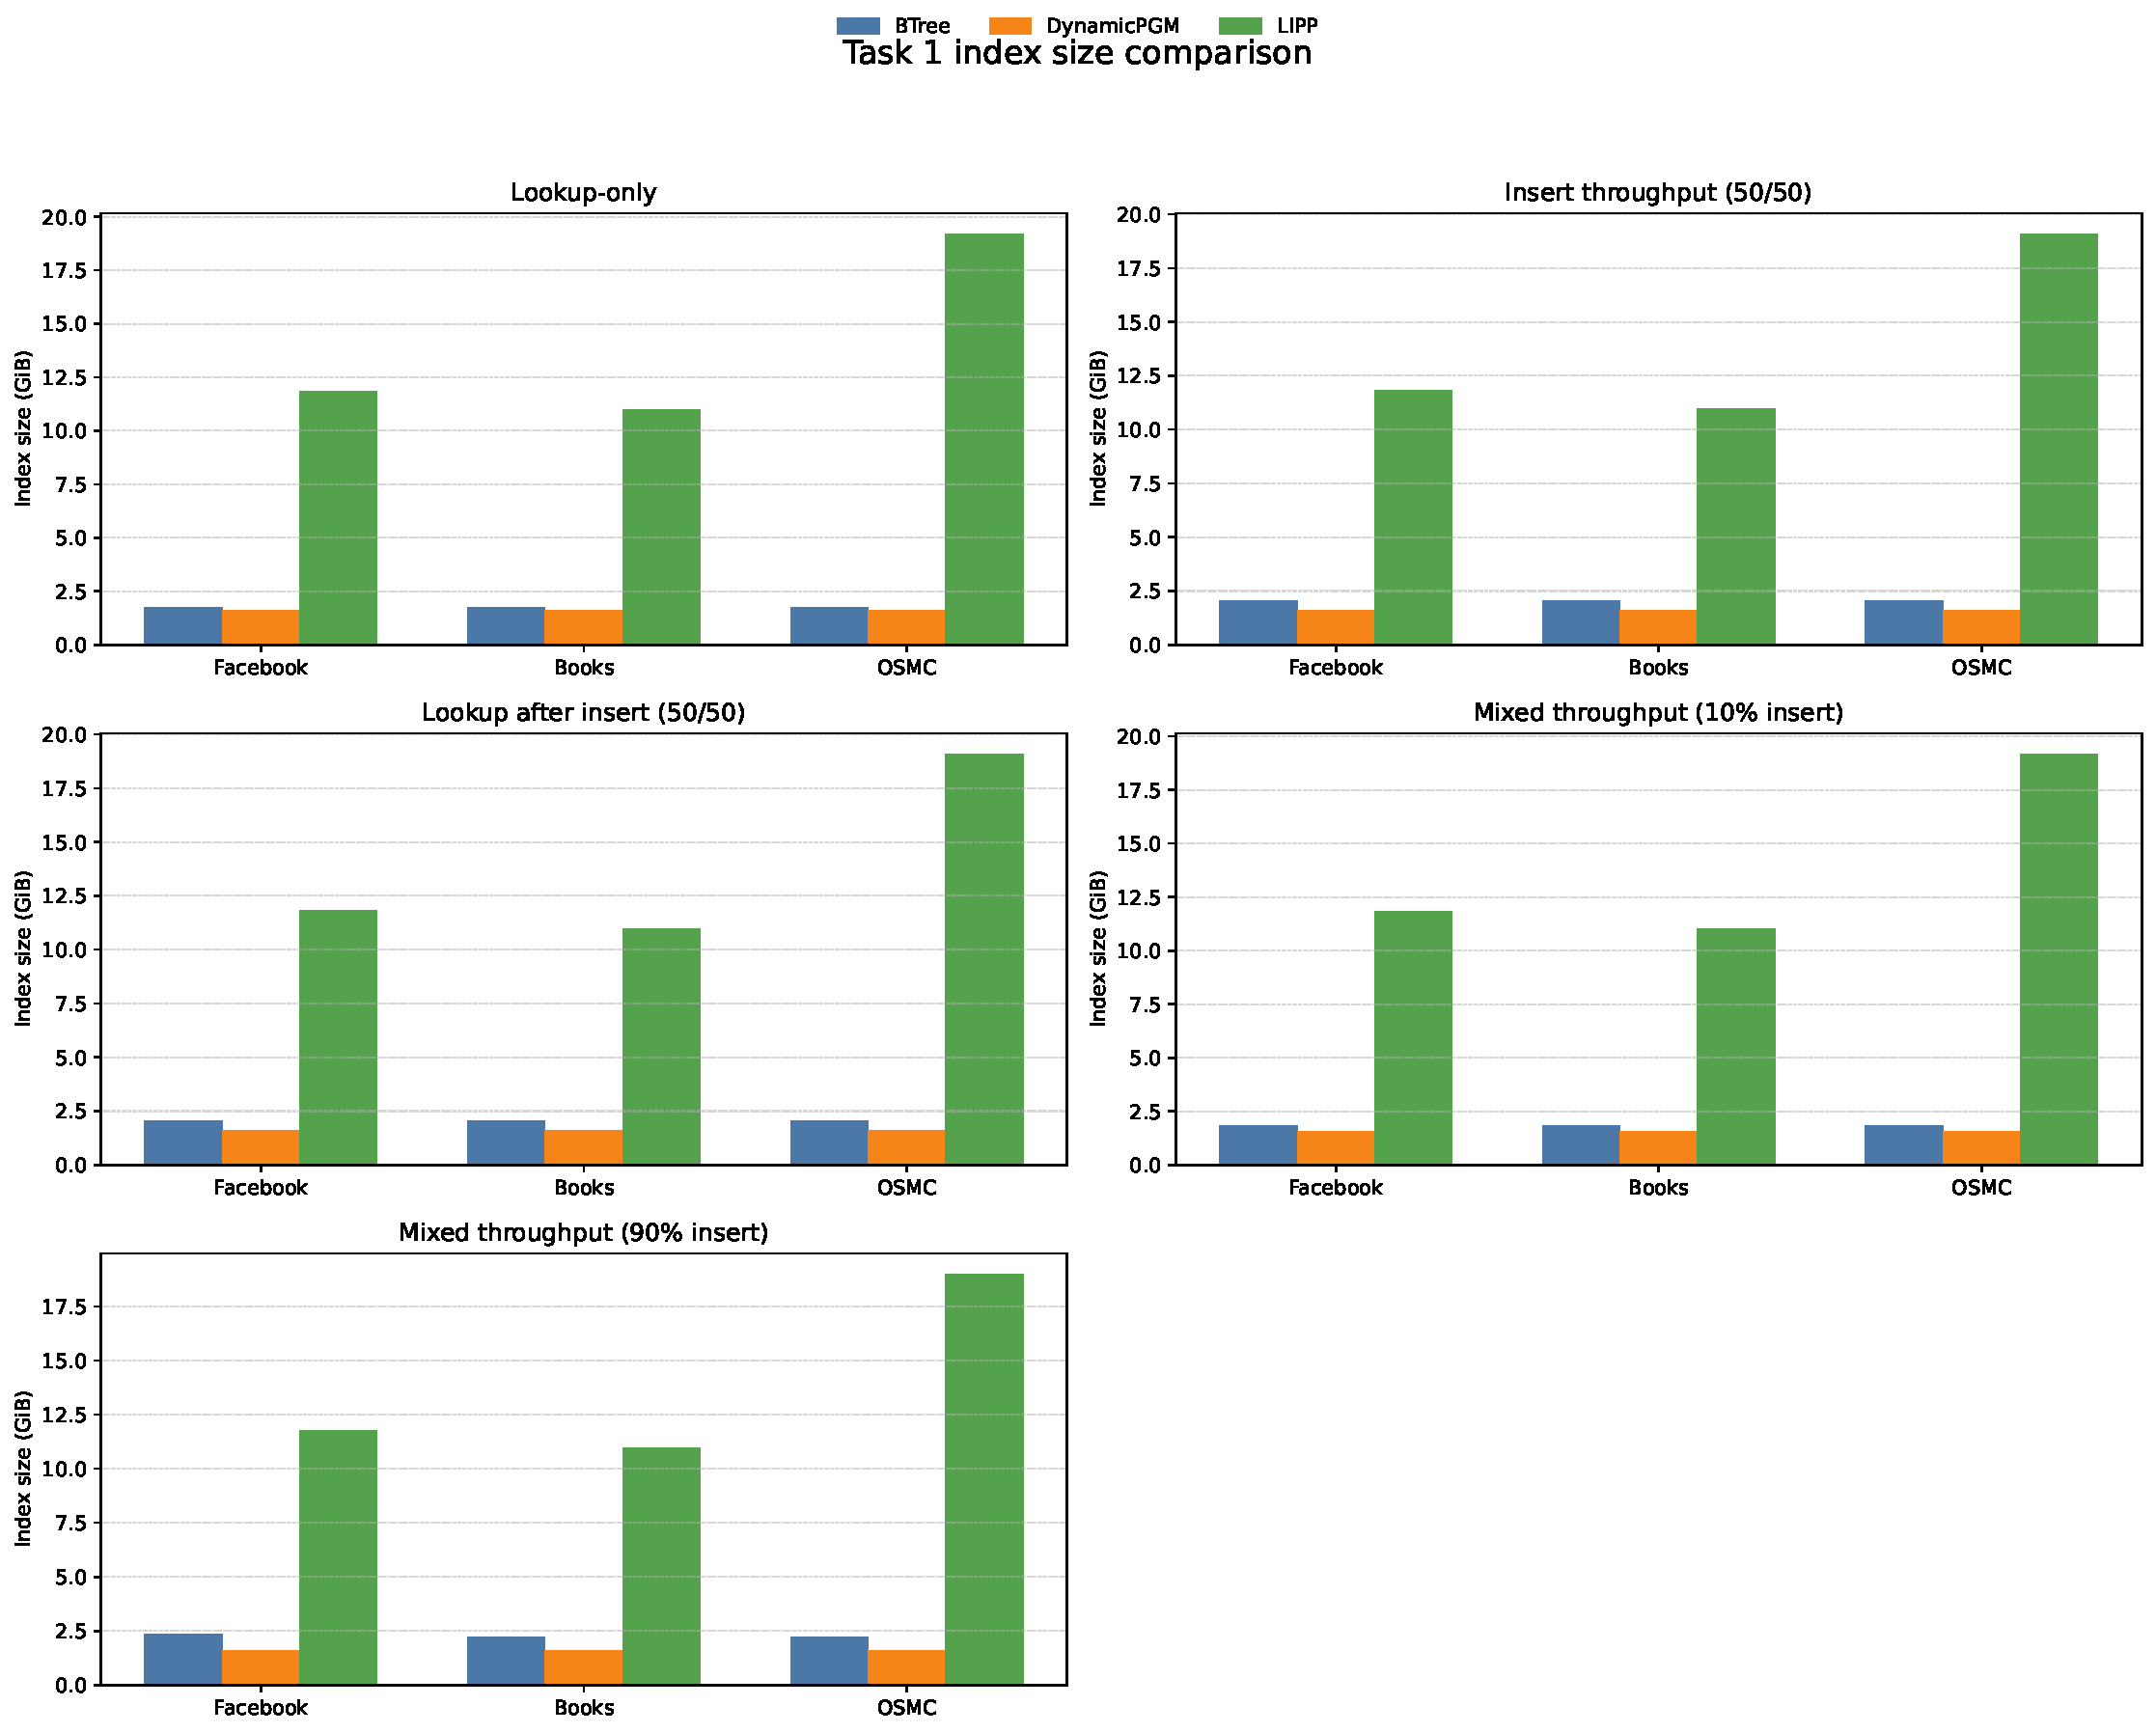
\includegraphics[width=\textwidth]{figures/task1_index_size_overview.png}
    \caption{Index size comparison for the selected best-throughput configuration in each workload.}
    \label{fig:size}
\end{figure}

\section{Why the performance differs}

\subsection{Why LIPP wins reads}
LIPP is designed to predict precise positions within node arrays. In the repository
README, LIPP lookup is described as a model-guided traversal that can return directly
from a predicted slot, or recurse only when a collision has already been turned into a
child node. That design minimizes the corrective search work at lookup time.

The benchmark results match that expectation strongly:
\begin{itemize}[leftmargin=1.5em]
    \item lookup-only throughput is above \SI{300}{Mops/s} on all three datasets,
    \item post-insert lookup remains above \SI{250}{Mops/s} on all three datasets,
    \item even the 10\% insert mixed workload stays between \SI{10.447}{Mops/s} and
    \SI{17.526}{Mops/s}, well above the alternatives.
\end{itemize}

So the empirical story is that when the workload is dominated by lookups, the benefit of
direct model-based positioning outweighs the cost of maintaining LIPP's larger structure.

\subsection{Why DynamicPGM wins writes}
DynamicPGM supports updates using a buffered, amortized strategy rather than forcing each
insert to pay the full cost of maintaining exact placement. The README describes this as
a logarithmic method with buffers or auxiliary indexes of increasing size. That
architecture is exactly the kind of approach that should help insertion-heavy workloads.

Again the results line up with the design:
\begin{itemize}[leftmargin=1.5em]
    \item DynamicPGM is the winner for insert throughput in the 50/50 workload on every
    dataset, between \SI{5.332}{Mops/s} and \SI{6.192}{Mops/s}.
    \item DynamicPGM also wins every 90\% insert mixed workload, where it reaches
    \SI{2.663}{Mops/s} to \SI{2.972}{Mops/s}.
\end{itemize}

The downside is visible in the read side: once lookups dominate, DynamicPGM's need for
approximate prediction plus corrective searching leaves it far behind LIPP.

\subsection{Why BTree sits in the middle}
BTree is a classical balanced search tree. It does not have LIPP's extremely fast
learned direct-slot lookup, but it also does not depend on DynamicPGM's buffered
rebuild-and-merge update strategy. That makes it predictable and relatively stable, but
not best-in-class for either extreme.

Across the five workload metrics, BTree remains clustered around:
\begin{itemize}[leftmargin=1.5em]
    \item roughly \SI{1.7}{Mops/s}--\SI{2.1}{Mops/s} for lookup-heavy cases,
    \item roughly \SI{1.0}{Mops/s} for insert-heavy cases.
\end{itemize}

That stability may still be attractive as a baseline, but the Task 1 results show that
it gives up too much performance relative to the better-specialized learned indexes.

\subsection{How dataset properties affect the outcomes}
The winner pattern stays consistent across Facebook, Books, and OSMC, which is itself an
important finding: the ordering of methods is driven more by workload mix than by the
choice of dataset. Still, the dataset does affect the magnitude of the gains:
\begin{itemize}[leftmargin=1.5em]
    \item LIPP's lookup-only throughput is highest on Books
    (\SI{361.350}{Mops/s}) and lowest on OSMC (\SI{307.095}{Mops/s}).
    \item In the post-insert lookup metric, OSMC is also LIPP's weakest dataset
    (\SI{253.168}{Mops/s}), suggesting that this distribution is harder for LIPP's
    update-maintained structure than Facebook or Books.
    \item DynamicPGM's insertion throughput remains strong on all three datasets, but it
    is slightly lower on OSMC than on Facebook or Books.
\end{itemize}

The OSMC result also shows the highest run-to-run variability for LIPP after inserts.
That does not change the ranking, but it is a useful caution when interpreting averages.

\section{Best hyperparameters selected from the recorded runs}

Task 1 requires choosing the best hyperparameter setting for BTree and DynamicPGM rather
than averaging across all variants. Table~\ref{tab:hyperparameters} records the winning
configuration from the committed CSVs for each dataset/workload pair.

\begin{table}[H]
    \centering
    \caption{Best hyperparameter setting selected for each dataset/workload pair.}
    \label{tab:hyperparameters}
    \footnotesize
    \begin{tabular}{lll}
\toprule
Dataset / Workload & Best BTree configuration & Best DynamicPGM configuration \\
\midrule
Facebook / Lookup-only & LinearSearch / 8 & LinearSearch / 16 \\
Facebook / Insert throughput (50/50) & LinearSearch / 8 & ExponentialSearch / 256 \\
Facebook / Lookup after insert (50/50) & LinearSearch / 8 & ExponentialSearch / 256 \\
Facebook / Mixed throughput (10\% insert) & LinearSearch / 8 & BinarySearch / 64 \\
Facebook / Mixed throughput (90\% insert) & LinearSearch / 6 & BinarySearch / 128 \\
\midrule
Books / Lookup-only & LinearSearch / 8 & LinearSearch / 16 \\
Books / Insert throughput (50/50) & LinearSearch / 8 & InterpolationSearch / 512 \\
Books / Lookup after insert (50/50) & LinearSearch / 8 & InterpolationSearch / 512 \\
Books / Mixed throughput (10\% insert) & LinearSearch / 8 & LinearSearch / 32 \\
Books / Mixed throughput (90\% insert) & LinearSearch / 8 & LinearSearch / 32 \\
\midrule
OSMC / Lookup-only & LinearSearch / 8 & LinearSearch / 16 \\
OSMC / Insert throughput (50/50) & LinearSearch / 8 & LinearSearch / 1024 \\
OSMC / Lookup after insert (50/50) & LinearSearch / 8 & BinarySearch / 1024 \\
OSMC / Mixed throughput (10\% insert) & LinearSearch / 8 & BinarySearch / 64 \\
OSMC / Mixed throughput (90\% insert) & LinearSearch / 8 & BinarySearch / 128 \\
\bottomrule
\end{tabular}

\end{table}

Two broad trends emerge:
\begin{itemize}[leftmargin=1.5em]
    \item BTree almost always prefers \texttt{LinearSearch} with value 8, except for the
    Facebook 90\% insert workload where value 6 wins.
    \item DynamicPGM prefers small values for lookup-only (16 on all datasets), while
    insertion-heavy workloads prefer larger values such as 32, 64, 128, 256, 512, or
    1024 depending on dataset and search method.
\end{itemize}

This is consistent with the intuition that DynamicPGM can trade lookup precision for
better update behavior under insertion-heavy conditions.

\section{Detailed Task 1 summary}

Task 1 serves as the empirical foundation for the rest of the project. The main point of
the milestone is not just to produce bar plots, but to understand the workload-dependent
strengths and weaknesses of the baseline indexes before attempting a hybrid design in
Task 2.

The detailed summary of what was accomplished is:
\begin{enumerate}[leftmargin=1.5em]
    \item set up the minimal Task 1 benchmark pipeline from the repository scripts,
    \item generated the prescribed workloads for all three datasets,
    \item benchmarked BTree, DynamicPGM, and LIPP with three repeats,
    \item evaluated multiple BTree and DynamicPGM hyperparameter settings and selected
    the best-performing one for each case,
    \item aggregated results into per-workload summaries,
    \item interpreted the measurements in terms of the underlying index designs.
\end{enumerate}

The final Task 1 conclusion is straightforward:
\begin{itemize}[leftmargin=1.5em]
    \item choose \textbf{LIPP} for lookup-dominated workloads when memory overhead is
    acceptable,
    \item choose \textbf{DynamicPGM} for insertion-dominated workloads,
    \item use \textbf{BTree} as a stable classical baseline rather than the best option
    for peak throughput.
\end{itemize}

That conclusion directly motivates the Task 2 project direction: if DynamicPGM is best at
absorbing inserts and LIPP is best at serving lookups, then a hybrid design may be able
to combine their strengths if the migration or flushing cost can be controlled.

\section{Conclusion}

Using the committed Task 1 benchmark artifacts in this repository, we compared BTree,
DynamicPGM, and LIPP across the Facebook, Books, and OSMC datasets and across the four
required workloads. The measured results are highly consistent:
\begin{itemize}[leftmargin=1.5em]
    \item LIPP is by far the fastest for lookup-heavy workloads,
    \item DynamicPGM is the fastest for insertion-heavy workloads,
    \item BTree is consistent but does not win either extreme,
    \item DynamicPGM is the most space-efficient,
    \item LIPP achieves its read performance with a much larger index footprint.
\end{itemize}

These results provide the right baseline for the next stage of the assignment. They show
exactly why a hybrid DynamicPGM+LIPP design is attractive: the two learned indexes win
different workload regimes, and the remaining challenge is whether their strengths can be
combined without paying too much migration overhead.

\end{document}
